
\section{Directional Derivative}

	\begin{frame}{Directional derivative}
		\begin{itemize}
			\item The directional derivative basically states how a function changes along a certain direction
			\item We can use it to linearise a nonlinear function , which gives us our Newton Rhapson method
			\item Finding the changes of a functional \footnote{Function of functions} with respect to its corresponding functions. This is akin to the variational or virtual work theorems
			\item The directional derivative gives the linear change!!! So at a point in the domain, it gives the linear change (Gradients) in a certain direction
			
		\end{itemize}
	\end{frame}


	\begin{frame}
		\begin{figure}
			\centering
			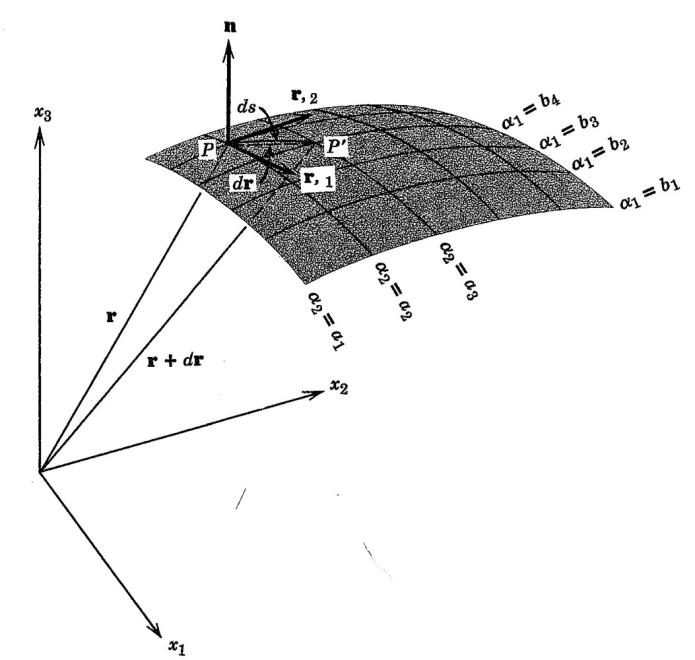
\includegraphics[width=1\linewidth]{\pth/function/fig1}
			\label{fig:fig3}
		\end{figure}
		\begin{itemize}
			\item So we have a funcitonal which depends on differerent functions or $\ve{x}$
			\item We cut the function with a plane (Blue) which gives us a curve how the function changes along that direction
			\item Finding that linear change along the direction ${u}$ \footnote{Remember that $u$ is a unit vector} gives the directional derivative. See that the curve is now dependant on $\epsilon$
			
			\item It is denoted as $\nabla_u$ or $D f(\ve{x})[u]$
			
		\end{itemize}
	\end{frame}

	\begin{frame}{Example \#1}
		\begin{figure}
			\centering
			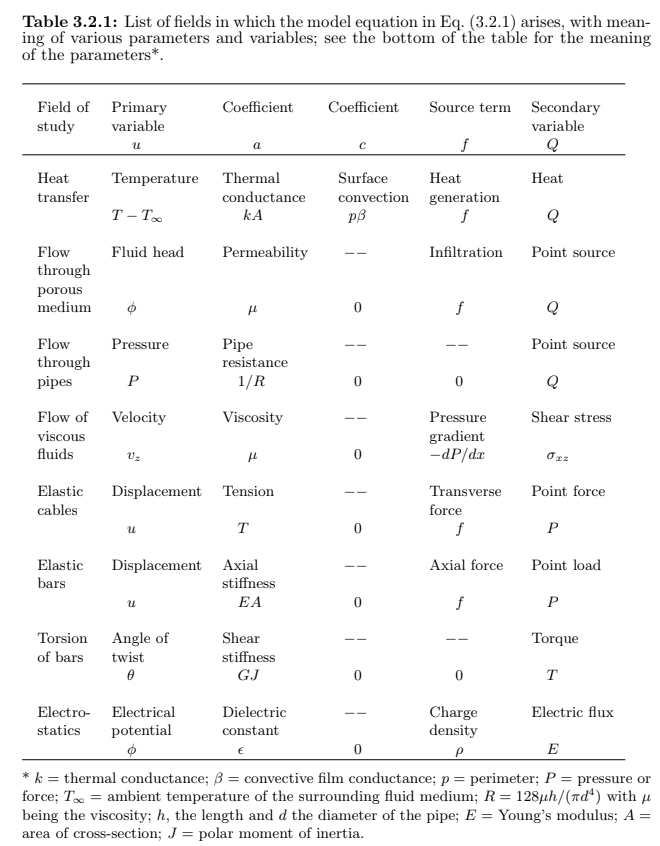
\includegraphics[width=0.5\linewidth]{\pth/function/fig2}
			\label{fig:fig2}
		\end{figure}
		\begin{itemize}
			\item Potential energy of the structure is
			\begin{align*}
				f(\ve{x}) = \frac{1}{2}kx_1^2 + \frac{1}{2}k(x_2-x_1)^2 - Fx_2 \\
				f(\ve{x+u}) = \frac{1}{2}k(x_1+u_1)^2 + \frac{1}{2}k(x_2 + u_2-x_1-u_1)^2 - F(x_2 + u_2) \\ 
				Df(\ve{x})[\ve{u}] \approx f(\ve{x+u}) - f(\ve{x}) 			
			\end{align*}	
			\item  Its approx $\approx$ as we want only the linear change, this is also what we mean when we write $\delta$f in variational calculus		
		\end{itemize}
	\end{frame}

	\begin{frame}
		\begin{itemize}
			\item How do we get the linear function? Taylor series!
			\begin{align*}
			f(\ve{x+\epsilon u}) = \frac{1}{2}k(x_1+\epsilon u_1)^2 + \frac{1}{2}k(x_2 + \epsilon u_2-x_1-\epsilon u_1)^2 - F(x_2 + \epsilon u_2) \\ 
			Df(\ve{x})[\ve{u}] \approx f(\ve{x+u}) - f(\ve{x}) \left(\text{Approx as only the linear change} \right)			
			\end{align*}
			\item This is the function on the plane that cuts the surface given in terms of $\epsilon$
			\item Linearise it about the point we get (And ignoring higher order terms)
			\begin{align*}
				f(\ve{x+\epsilon u}) = f(\ve{x}) + \left(\frac{ d}{ d\epsilon}|_{\epsilon = 0} f(\ve{x+\epsilon u}) \right) \epsilon + O(\epsilon^2)
			\end{align*}
			\item So our potential energy becomes , Take $\epsilon =1$ for unit direction
			\begin{align*}
			Df(\ve{x})[\ve{u}] = \left(\frac{ d}{ d\epsilon}|_{\epsilon = 0} f(\ve{x+\epsilon u}) \right) \\
			= \frac{ d}{ d\epsilon}|_{\epsilon = 0}\left(  \frac{1}{2}k(x_1+\epsilon u_1)^2 + \frac{1}{2}k(x_2 + \epsilon u_2-x_1-\epsilon u_1)^2 - F(x_2 + \epsilon u_2) \right) \\
			=k_1x_1u_1 + k(x_2-x_1)(u_2-u_1) - Fu_2 \\
			= \ve{u^T(Kx-F)}
			\end{align*}
		\end{itemize}
	\end{frame}

	\begin{frame}{Insight}
		\begin{itemize}
			\item So we get the form $\ve{u^T(Kx-F)}$ for some direction $\vec{u}$
			\item Equilbrium is satisfied when the potential is minimum for any $\vec{u}$ So $Df(x)[u] =0$
			\item This is exactly like the variational principle where we get something like $Df(x)[\delta u] =0$
			\item Where the Equilibrium has to be zero  $\ve{(Kx-F)}$ and therefore any work done on it by any displacment is zero ("Virtual displcament theory")
			\item At equilibrium the work done by the external and internal loads is equal to zero
			\item The functional may be still nonlinear with respect to $\ve{x}$ but we are linearising the function with respect to the change or direction $\ve{u}$ 
		\end{itemize}
	\end{frame}

	\begin{frame}
		 We can find the directional derivative of different things like the determinant of a matrix etc. Check Bonet Page 16
	\end{frame}